% !TEX TS-program = xelatex
% !TEX encoding = UTF-8 Unicode

\documentclass[a4paper,11pt]{article}
\usepackage{xeCJK}
\setCJKmainfont{IPAexMincho}
\setCJKsansfont{IPAexGothic}
\setCJKmonofont{IPAexGothic}
\usepackage[a4paper,margin=25mm]{geometry}
\usepackage{parskip}               % 段落間の余白
\setlength{\parindent}{0pt}        % 行頭インデントなし
\usepackage{enumitem}
\setlist[itemize,1]{label=・, left=0pt, nosep}
\usepackage{titlesec}
\usepackage{listings}
\usepackage{xcolor}
\usepackage[dvipdfmx]{graphicx}
\usepackage{float}


\lstset{
  language=Python,
  basicstyle=\ttfamily\small,
  breaklines=true,
  columns=fullflexible,
  inputencoding=utf8,
  keywordstyle=\color{blue},
  commentstyle=\color{gray},
  stringstyle=\color{teal},
  showstringspaces=false,
}
\titlespacing*{\subsection}{0pt}{9ex}{1ex}

\begin{document}

%―――――――――――――――――――――――――――――――――――――――
% タイトルブロック
\begin{center}
  {\LARGE \bfseries ウェアラブル端末と心理入力アプリデータを統合した\\感情予測アルゴリズムの開発}\\[6ex]
\end{center}

\hrule\vspace{1ex}
{\normalsize 2025-06-13 進捗報告 \hfill 森雄大}\\
\hrule\vspace{5ex}



%―――――――――――――――――――――――――――――――――――――――
% データ収集・解析の概要
\subsection*{感情スコアの時間傾向}
線形混合モデル(Linear Mixed Model, LMM)を使い、目的変数である感情スコアを固定効果とランダム効果で説明するモデルを構築した。

\vspace{2ex}
\noindent \textbf{【データ構造】}

感情スコアデータ一つ一つに、計測した時間帯カテゴリ(例:00:00–03:00)と被験者IDを紐づけ、データを被験者グループ単位で扱えるようにした。

\vspace{2ex}
\noindent \textbf{【モデル構造】}

\begin{itemize}
\item 固定効果:全被験者に共通した時間帯カテゴリの効果
\item ランダム効果:被験者ごとのベースラインの個人差
\end{itemize}

\vspace{2ex}
\noindent \textbf{【結果の解釈】}

\begin{itemize}
\item 固定効果:被験者個人差を除いた時間帯別の平均的なArousal・Valenceスコア
\item ランダム効果の分散:被験者間のベースラインの個人差の程度
\end{itemize}

arousal ~ 1 + timeBin + (1|subjectId)

valence ~ 1 + timeBin + (1|subjectId)


\subsection*{感情スコアの可視化}
時間帯による感情スコアの傾向を追うため、全感情計測データを時間帯カテゴリ別にプロットした(図1・2)。

\vspace{1ex}
\noindent \textbf{【注意】} 感情スコアが0–10の整数値のため、データポイントが重ならないよう±0.5 のジッタリングを適用している。

\begin{figure}[H]
  \centering
  \begin{minipage}{0.4\columnwidth}
     \centering
     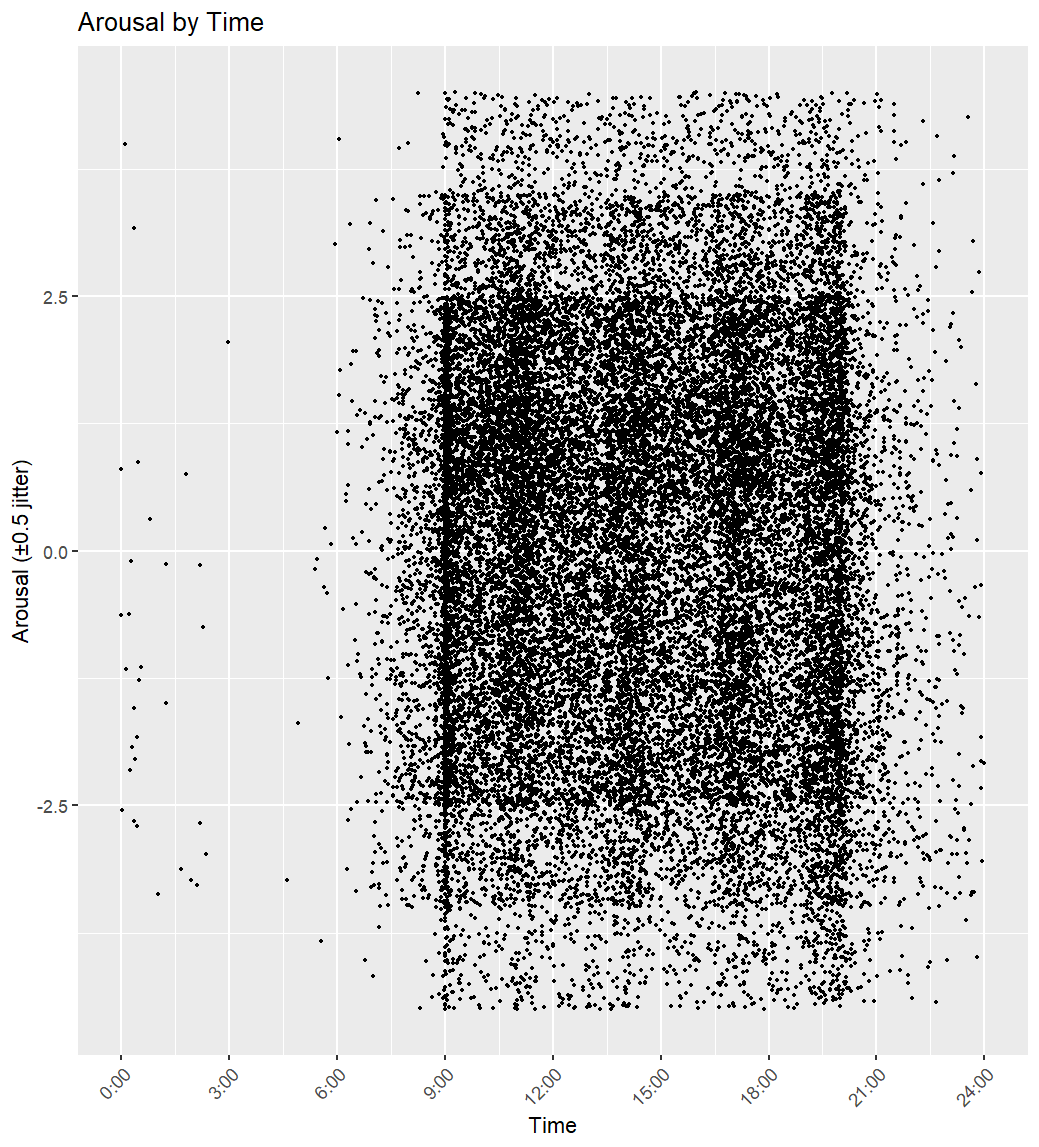
\includegraphics[width=\columnwidth]{/home/mori/projects/affective-forecast/R-workspace/arousal_by_time.png}
     \caption{Arousalの時間帯カテゴリ別分布(ジッタあり)\\y軸:Arousalスコア(0–10の整数値に±0.5ジッタ適用)}
  \end{minipage}
%
  \begin{minipage}{0.4\columnwidth}
     \centering
     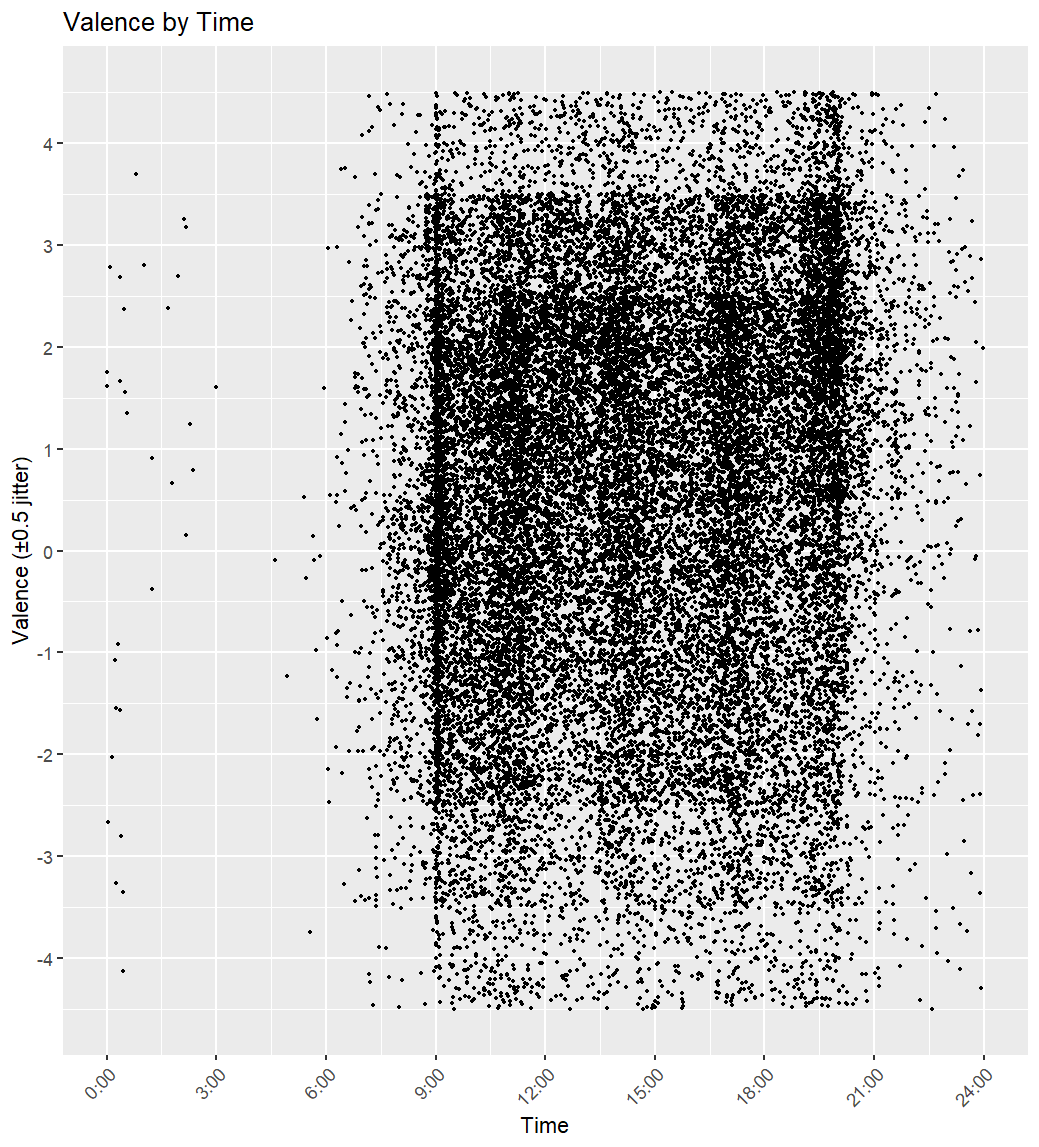
\includegraphics[width=\columnwidth]{/home/mori/projects/affective-forecast/R-workspace/valence_by_time.png}
     \caption{Valenceの時間帯カテゴリ別分布(ジッタあり)\\y軸:Valenceスコア(0–10の整数値に±0.5ジッタ適用)}
  \end{minipage}
\end{figure}

\subsection*{感情スコアの固定効果の可視化}
線形混合モデルで推定した固定効果(時間帯別の推定平均値)とその標準誤差を以下に示す(図3・4)。

\vspace{1ex}
\noindent \textbf{【読み方】} エラーバーは95%信頼区間を表し、バーが重ならない時間帯間には有意差がある可能性が高い。

\begin{figure}[H]
  \centering
  \begin{minipage}{0.4\columnwidth}
     \centering
     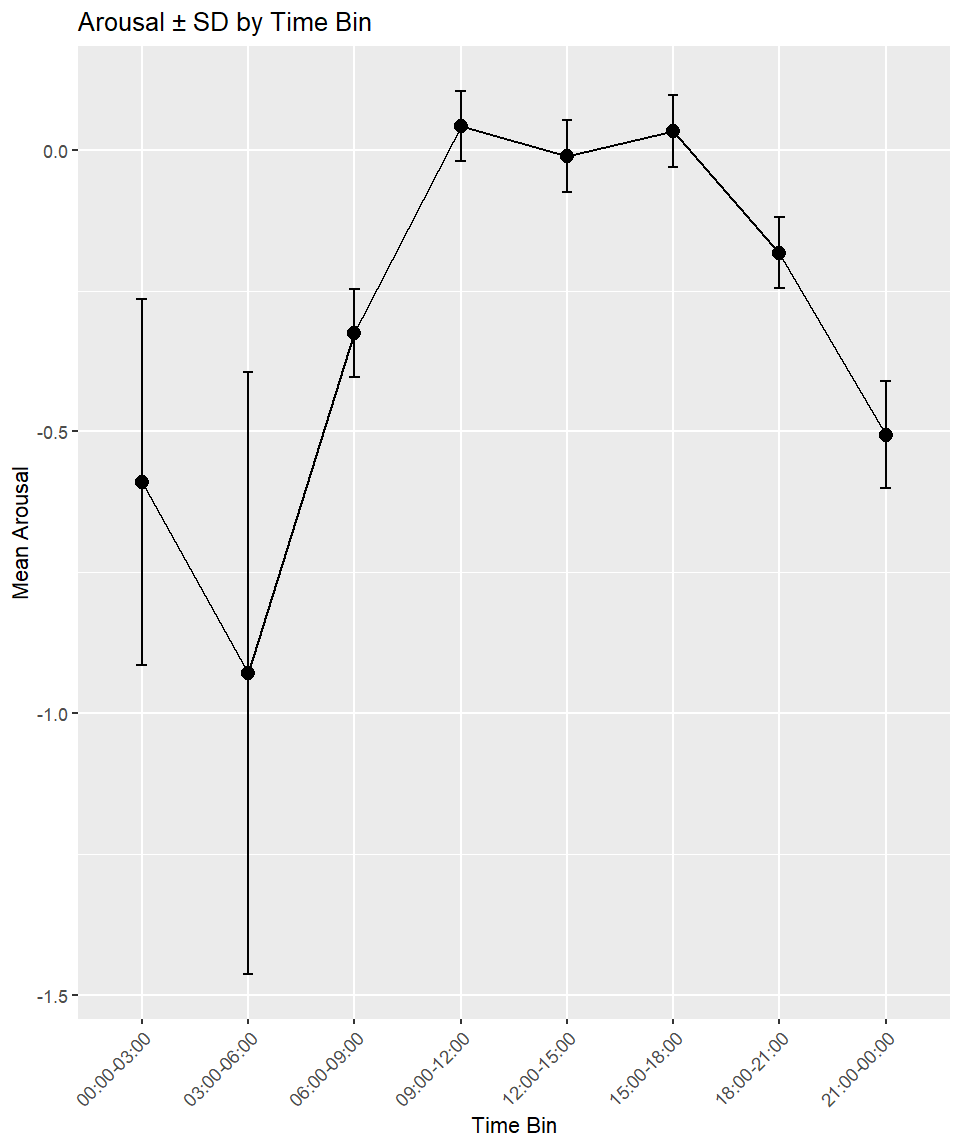
\includegraphics[width=\columnwidth]{/home/mori/projects/affective-forecast/R-workspace/arousal_by_timebin.png}
     \caption{時間帯別 Arousal の推定平均値(固定効果)および標準誤差(SE)}
  \end{minipage}
%
  \begin{minipage}{0.4\columnwidth}
     \centering
     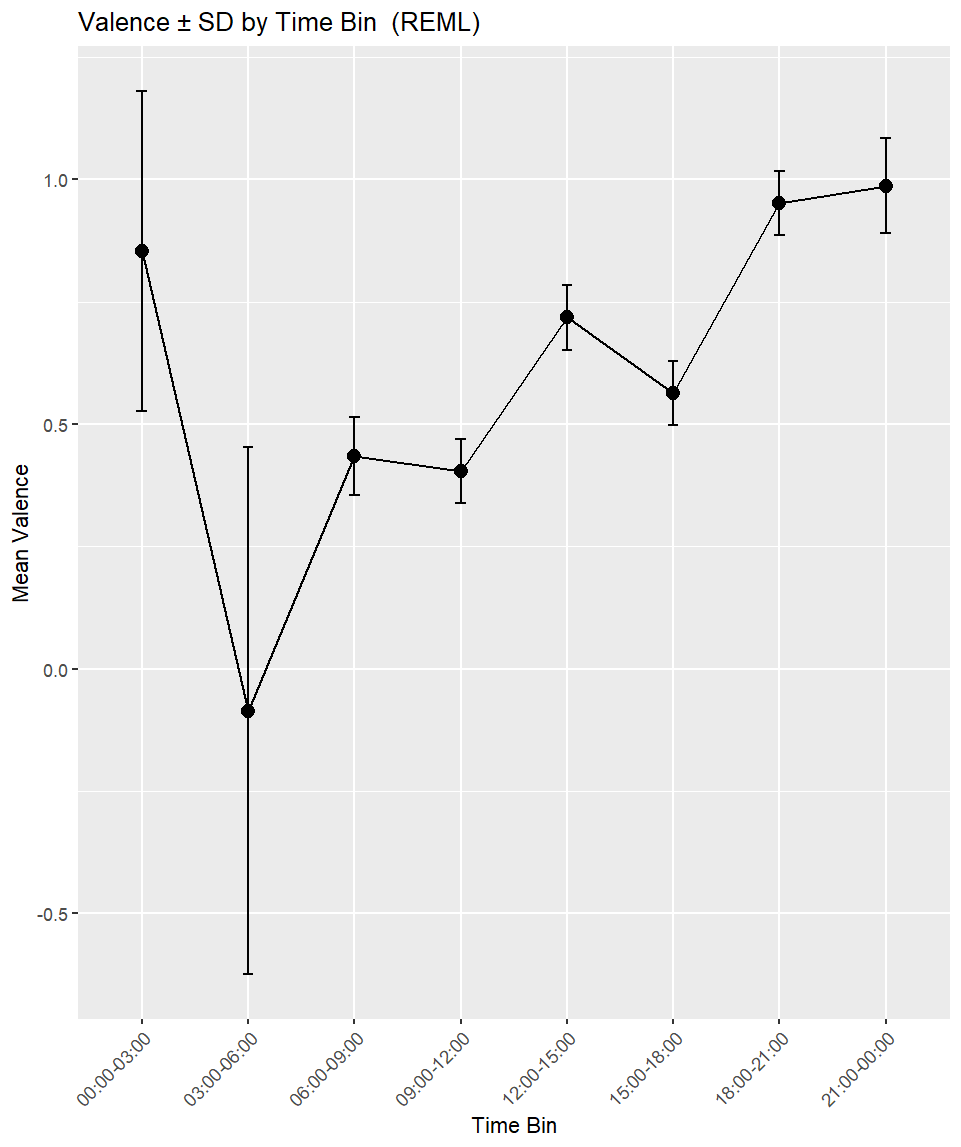
\includegraphics[width=\columnwidth]{/home/mori/projects/affective-forecast/R-workspace/valence_by_timebin.png}
     \caption{時間帯別 Valence の推定平均値(固定効果)および標準誤差(SE)}
  \end{minipage}
\end{figure}


\subsection*{その他メタデータをカテゴリ変数として考慮}
基本モデルでは時間帯のみを説明変数としていたが、被験者の個人特性(メタデータ)を追加することで、より精度の高い推定が可能か検討した。

\vspace{2ex}
\noindent \textbf{【追加したメタデータ】}

\begin{itemize}
\item 性別(男性・女性)

\item 年齢(10歳単位でカテゴリ化)

\item 楽観性(質問票の楽観的設問に対する平均スコアを四捨五入で1~4の整数化)

\item 悲観性(質問票の悲観的設問に対する平均スコアを四捨五入で1~4の整数化)

\end{itemize}

\vspace{2ex}
以下に、各メタデータを考慮したモデルの推定結果を示す。

\vspace{3ex}
\subsection*{モデル比較による効果の検証}

各メタデータを追加したモデルの性能をAIC(Akaike Information Criterion)で比較した。AICが小さいほど良いモデルであり、ベースモデル(①)からのΔAICで改善度を評価した。

\vspace{2ex}
\begin{table}[H]
\centering
\begin{tabular}{|c|l|r|r|r|r|}
\hline
モデル & 固定効果の追加 & AIC (arousal) & ΔAIC vs ① & AIC (valence) & ΔAIC vs ① \\
\hline
① & time\_bin & \textbf{115,599.8} & 0.0 & \textbf{116,106.1} & 0.0 \\
② & + gender & 115,601.7 & +1.9 & \textbf{116,103.0} & \textbf{−3.1} \\
③ & + age & 115,605.5 & +5.7 & 116,111.7 & +5.6 \\
④ & + mean\_optimism & 115,601.9 & +2.1 & 116,107.0 & +0.9 \\
⑤ & + mean\_pessimism & 115,604.9 & +5.1 & 116,110.4 & +4.3 \\
\hline
\end{tabular}
\caption{各メタデータを追加したモデルのAIC比較}
\end{table}

\vspace{2ex}
\noindent \textbf{【要点】}

\begin{itemize}
\item \textbf{valence}は②(+gender)でのみAICが有意に改善(−3.1)
\item それ以外はAICが上昇または微増で、情報量的には\textbf{追加メリットなし}
\item arousalについては、すべてのメタデータ追加でAICが悪化
\item 性別のみがvalence推定に有効な追加情報を提供
\end{itemize}

\vspace{3ex}
\subsubsection*{性別による効果}
\begin{figure}[H]
  \centering
  \begin{minipage}{0.4\columnwidth}
     \centering
     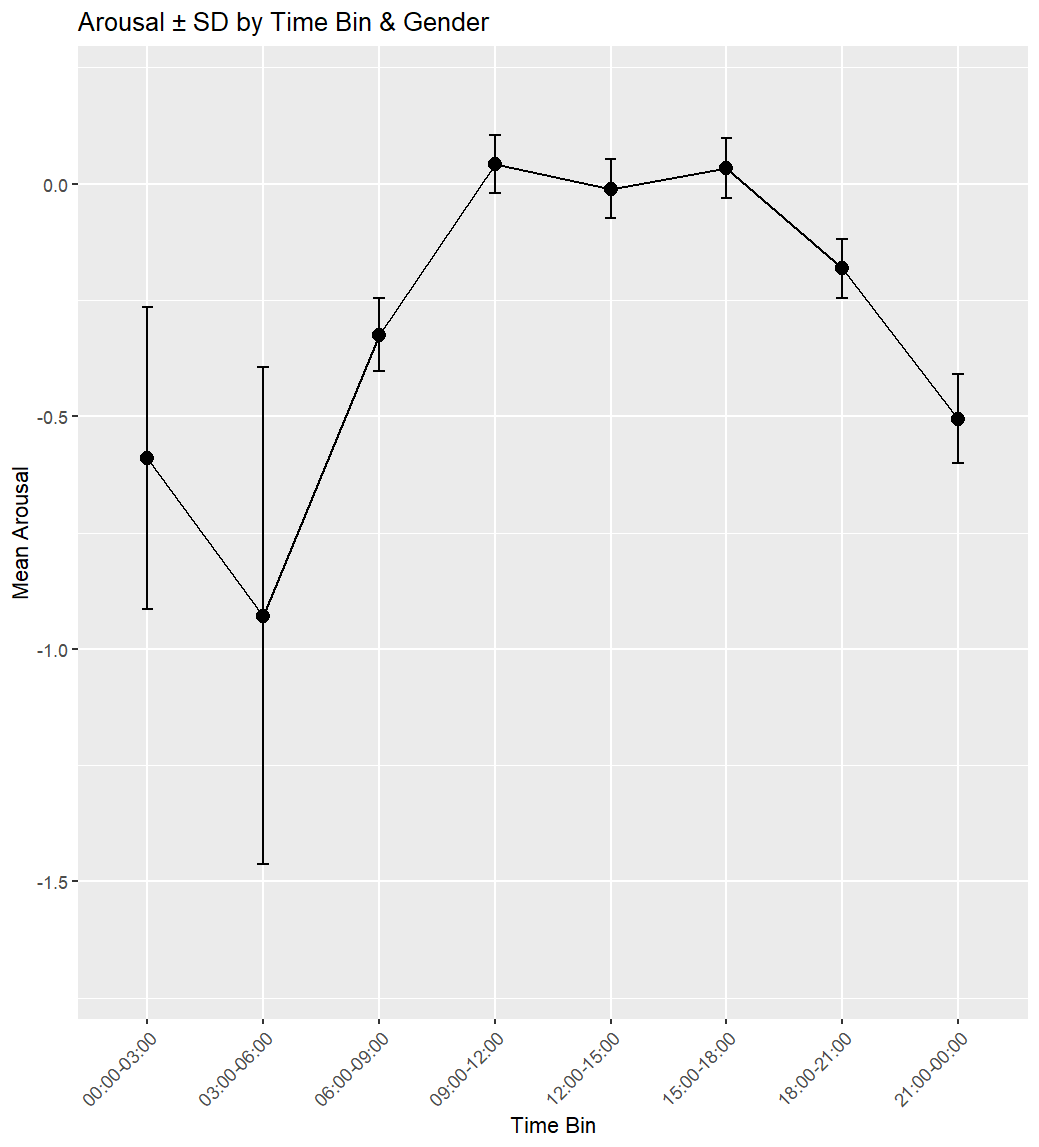
\includegraphics[width=\columnwidth]{/home/mori/projects/affective-forecast/R-workspace/arousal_by_timebin_and_gender.png}
     \caption{性別を考慮したArousal の推定平均値}
  \end{minipage}
%
  \begin{minipage}{0.4\columnwidth}
     \centering
     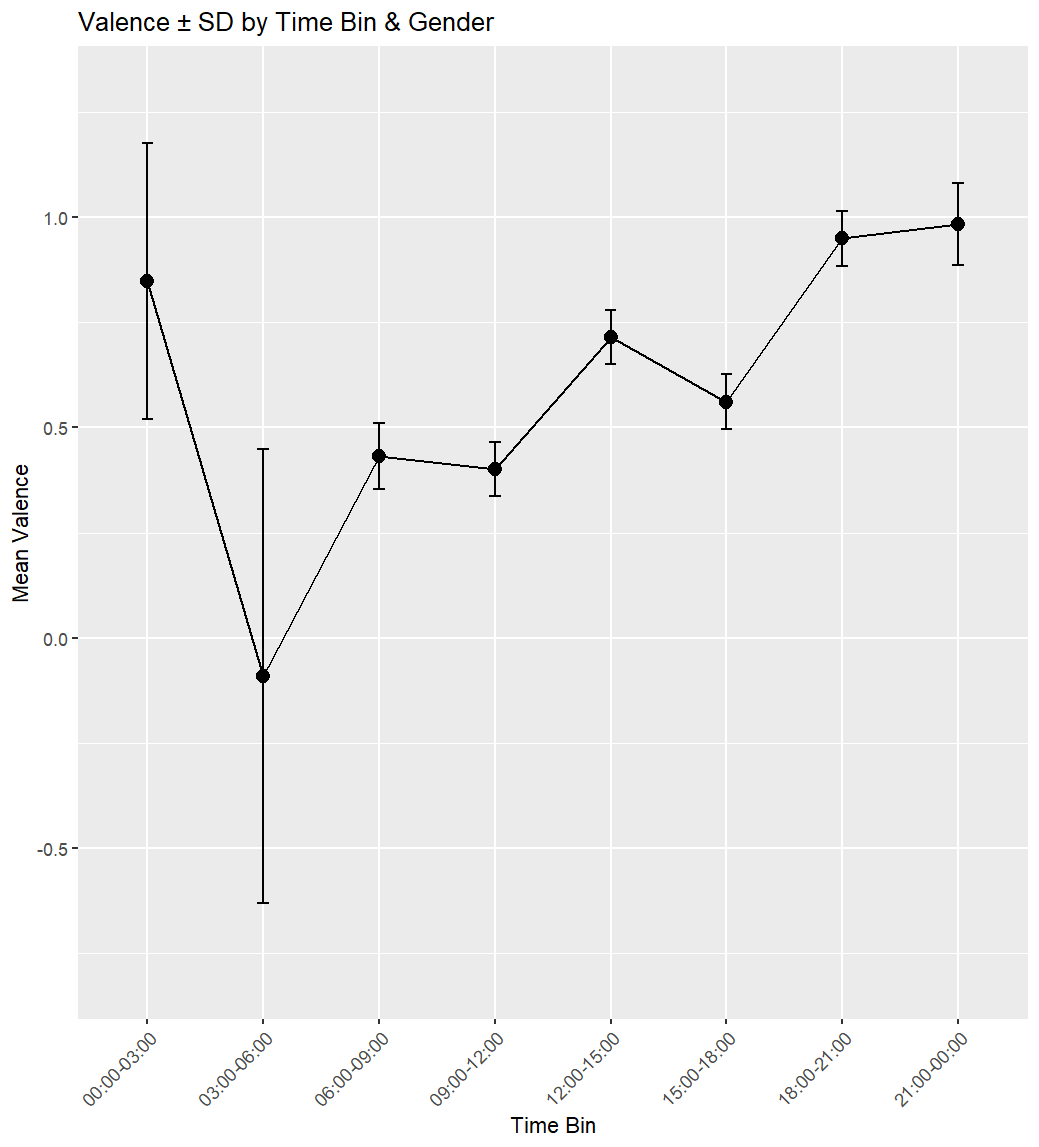
\includegraphics[width=\columnwidth]{/home/mori/projects/affective-forecast/R-workspace/valence_by_timebin_and_gender.png}
     \caption{性別を考慮したValence の推定平均値}
  \end{minipage}
\end{figure}

\vspace{3ex}
\subsubsection*{年齢による効果}
\begin{figure}[H]
  \centering
  \begin{minipage}{0.4\columnwidth}
     \centering
     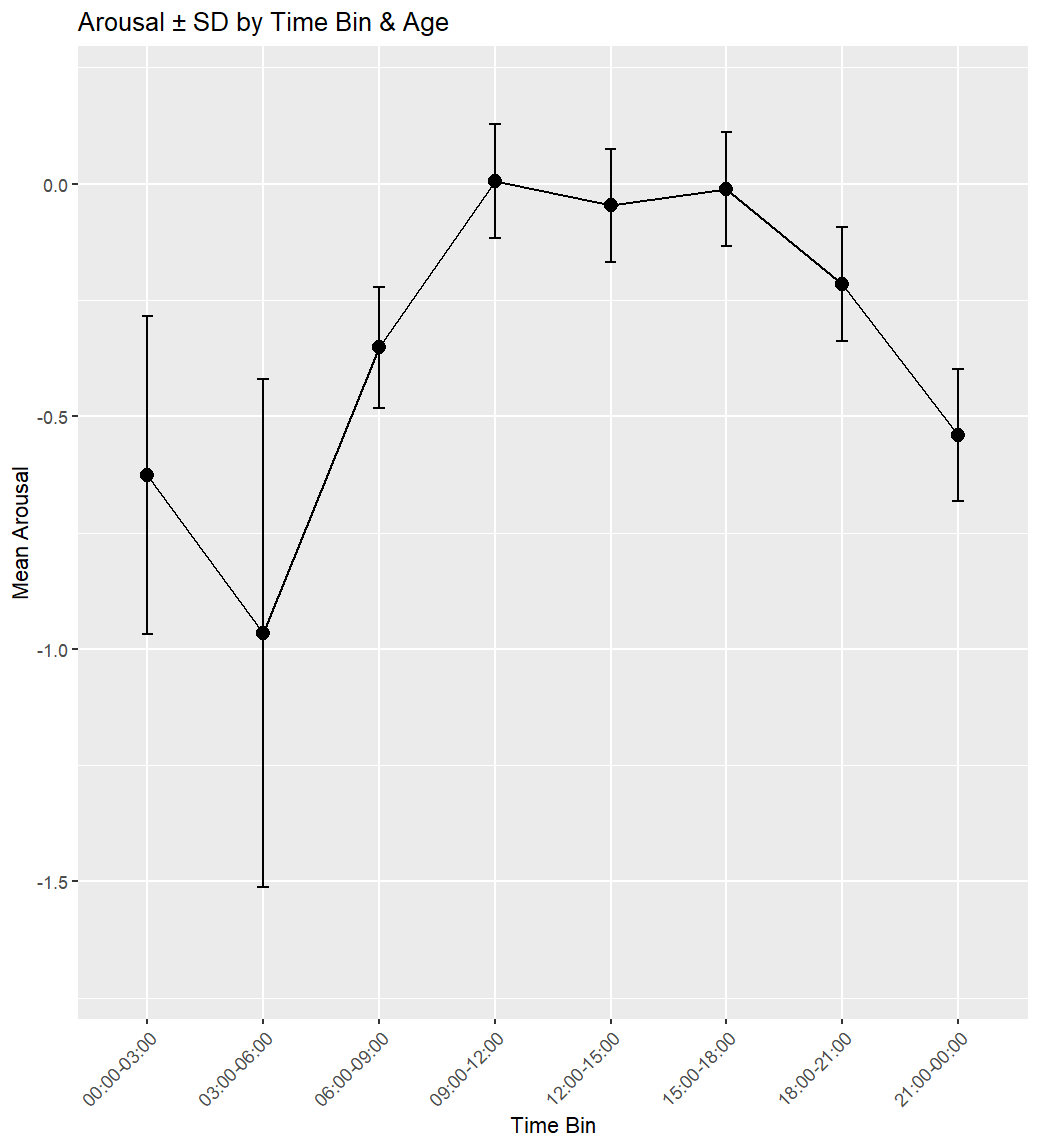
\includegraphics[width=\columnwidth]{/home/mori/projects/affective-forecast/R-workspace/arousal_by_timebin_and_age.png}
     \caption{年齢を考慮したArousal の推定平均値}
  \end{minipage}
%
  \begin{minipage}{0.4\columnwidth}
     \centering
     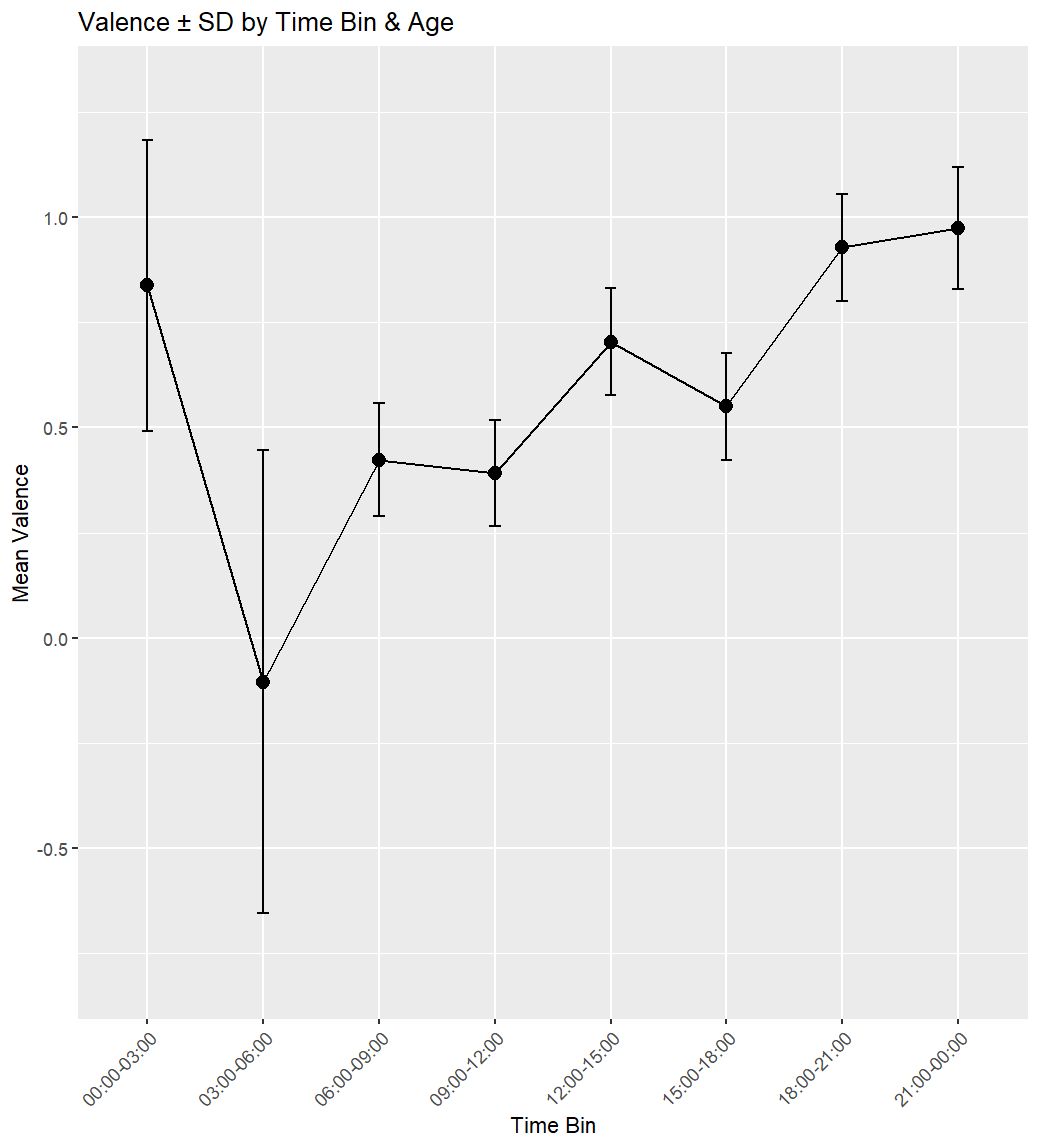
\includegraphics[width=\columnwidth]{/home/mori/projects/affective-forecast/R-workspace/valence_by_timebin_and_age.png}
     \caption{年齢を考慮したValence の推定平均値}
  \end{minipage}
\end{figure}

\vspace{3ex}
\subsubsection*{楽観性による効果}
\begin{figure}[H]
  \centering
  \begin{minipage}{0.4\columnwidth}
     \centering
     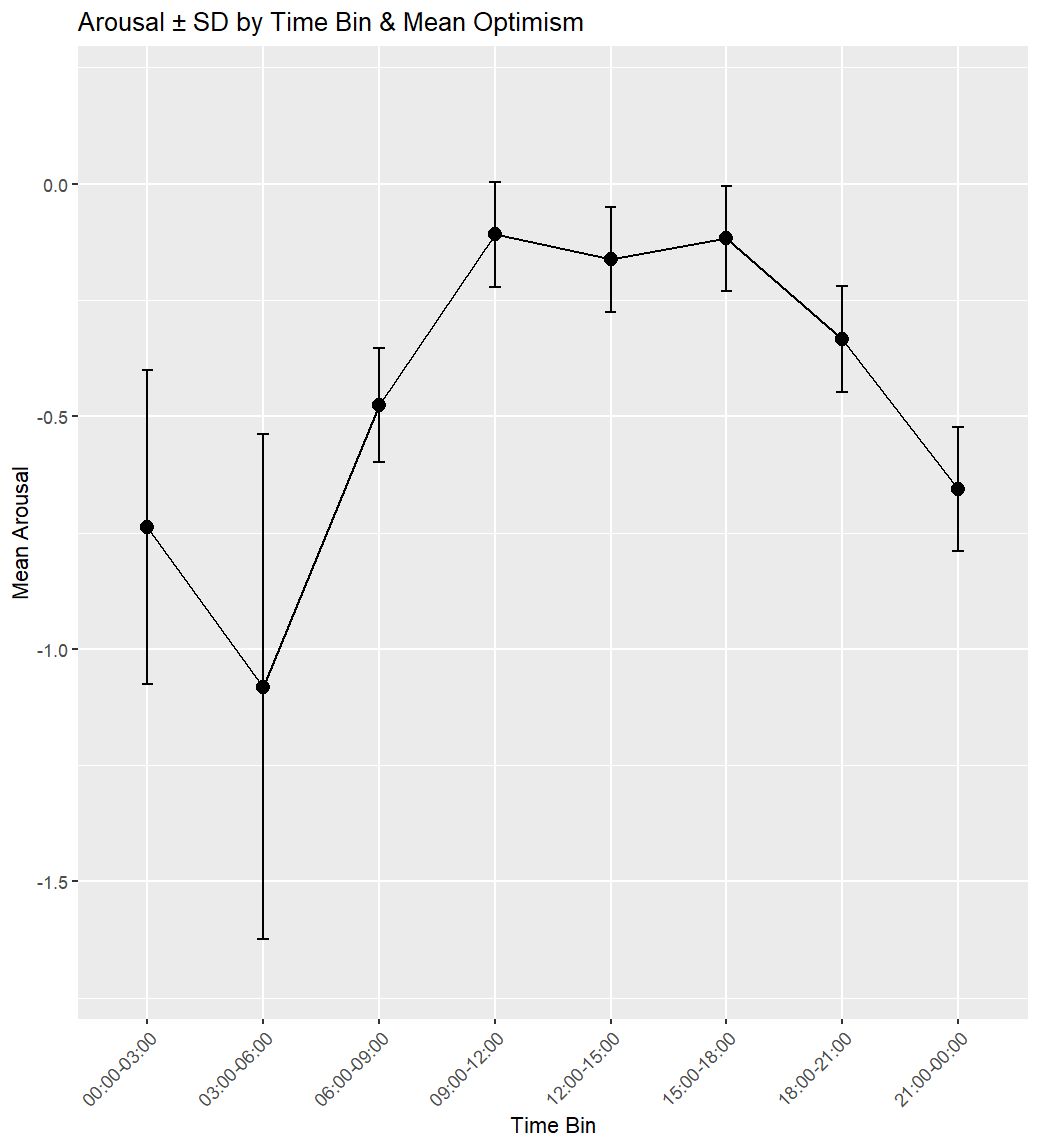
\includegraphics[width=\columnwidth]{/home/mori/projects/affective-forecast/R-workspace/arousal_by_timebin_and_meanoptimism.png}
     \caption{楽観性を考慮したArousal の推定平均値}
  \end{minipage}
%
  \begin{minipage}{0.4\columnwidth}
     \centering
     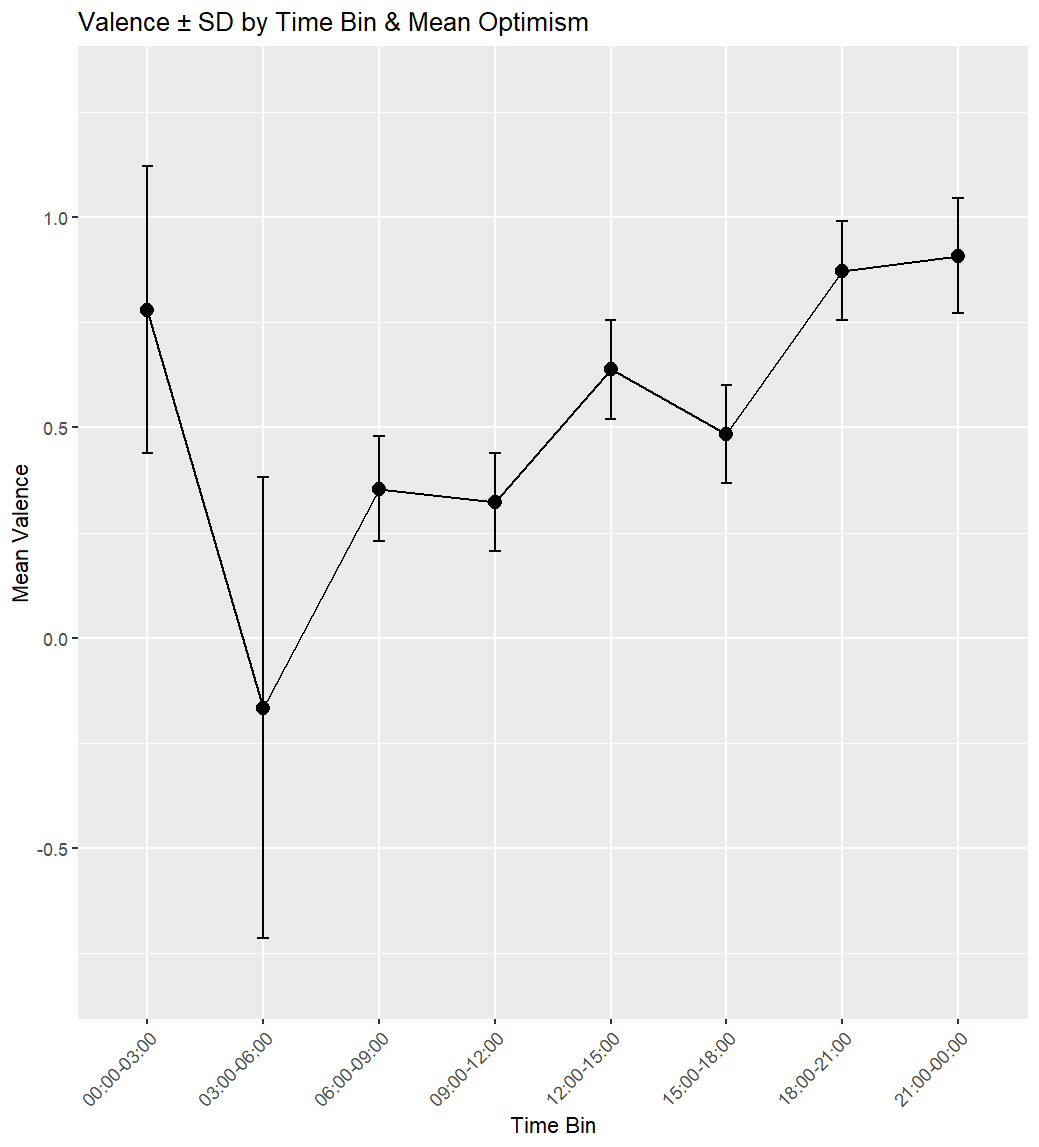
\includegraphics[width=\columnwidth]{/home/mori/projects/affective-forecast/R-workspace/valence_by_timebin_and_meanoptimism.png}
     \caption{楽観性を考慮したValence の推定平均値}
  \end{minipage}
\end{figure}

\vspace{3ex}
\subsubsection*{悲観性による効果}
\begin{figure}[H]
  \centering
  \begin{minipage}{0.4\columnwidth}
     \centering
     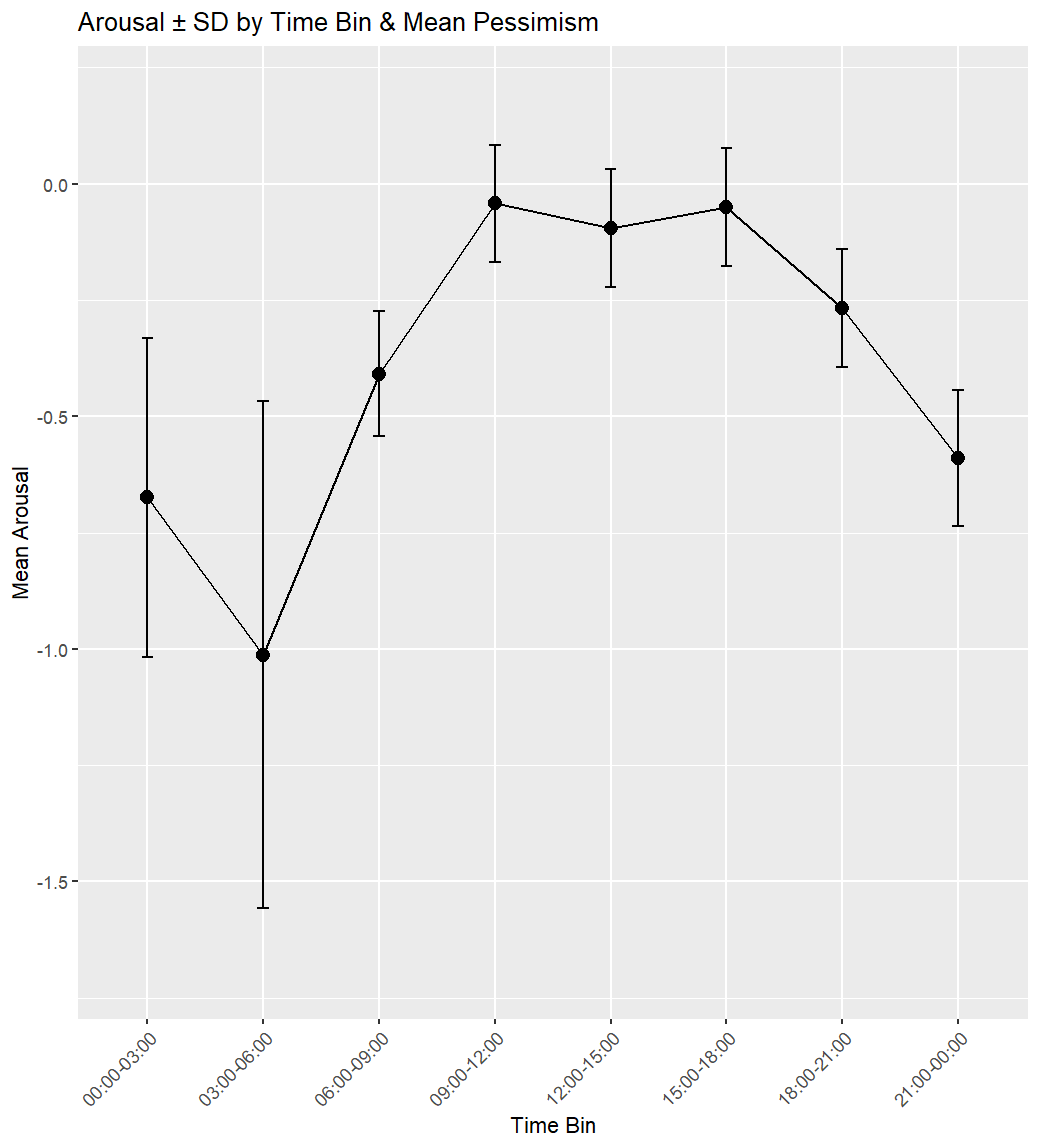
\includegraphics[width=\columnwidth]{/home/mori/projects/affective-forecast/R-workspace/arousal_by_timebin_and_meanpessimism.png}
     \caption{悲観性を考慮したArousal の推定平均値}
  \end{minipage}
%
  \begin{minipage}{0.4\columnwidth}
     \centering
     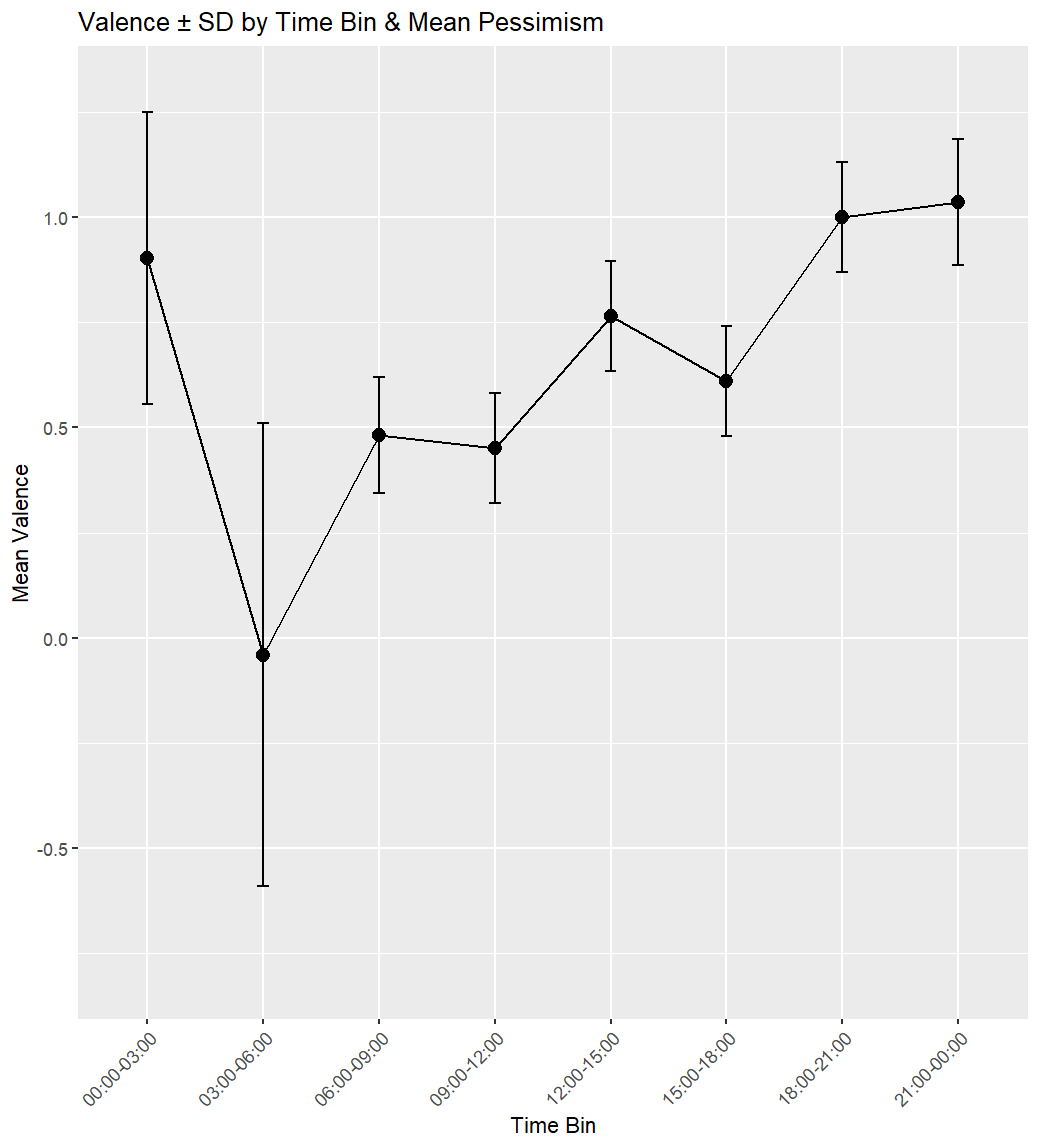
\includegraphics[width=\columnwidth]{/home/mori/projects/affective-forecast/R-workspace/valence_by_timebin_and_meanpessimism.png}
     \caption{悲観性を考慮したValence の推定平均値}
  \end{minipage}
\end{figure}




\end{document}
